% This is a comment.
% the region directly below this comment, up till the command \begin{document} is known as the 'preamble'
% basic setup
\documentclass{article}
\usepackage[english]{babel}
\usepackage[utf8]{inputenc}

% for mathematics
\usepackage{amsmath}
\usepackage{amsthm}
% define theorems, lemmas, etc
\newtheorem{theorem}{Theorem}
\newtheorem{lemma}{Lemma}
\newtheorem{corollary}{Corollary}
\newtheorem{definition}{Definition}
\newtheorem{example}{Example}
\usepackage{amssymb}

% for adjusting margins
\usepackage{geometry}
\geometry{
	a4paper,
 	left=26mm,
 	right=20mm,
 	top=33mm,
 	bottom=38mm
}

% for introducing urls
\usepackage{url}

% for colored text
\usepackage{color}

% for creating lists
\usepackage{enumerate}

% for import graphics
\usepackage{graphicx}

% include algorithm package
\usepackage[]{algorithm2e, setspace}

% change font to times new roman
%\usepackage{times}

% add padding to in between paragraphs
\setlength{\parskip}{1em}

% eliminate indent at start of paragraph
\setlength\parindent{0pt}

% title details
\title{QF4102 Financial Modelling and Computation Assignment 3}
%\date{}
\author{G01 Wang Zexin, Chen Penghao}

%~~~~~~~~~~~~~~~~~~~~~~~~~~~~~~~~~~~~~~~~~~~~~~~~~~~~~~~~~~~~~~~~~~~~~~~~~~~~~~
\begin{document}

% insert title
\maketitle
% make a new page
\newpage

\section{Transformed Black-Scholes PDE model}
Consider the \textbf{transformed} Black-Scholes PDE model:
\begin{equation*}
  \begin{cases}
    \frac{\partial u}{\partial t} + \frac{\sigma ^ {2}}{2}\frac{\partial ^ {2} u}{\partial x^{2}} + (r - q - \frac{\sigma^{2}}{2})\frac{\partial u}{\partial x} -ru = 0, & x \in (-\infty, \infty), t \in [0, T) \\
    u(x, T) = \varphi(x), & 
  \end{cases}
\end{equation*}

\subsection{Derivation of fully implicit scheme}
Evaluate partial derivatives at $(x_{n}^{i}, t_{n})$ where $t_{n} = n\Delta t, x_{n}^{i} = i\Delta x, n \in [0, \frac{T}{\Delta t}), i \in [-x_{max}, x_{max}], I_{max} = \frac{x_{max}}{\Delta x}$
$$ \text{Use the forward time finite difference formulae : } \left. \frac{\partial u}{\partial t} \right| _{(x_{n}^{i}, t_{n})} = \frac{u_{n+1}^{i} - u_{n}^{i}}{\Delta t} + O(\Delta t)$$
$$ \text{Use the centred space finite difference formulae : } \left. \frac{\partial u}{\partial x} \right| _{(x_{n}^{i}, t_{n})} = \frac{u_{n}^{i+1} - u_{n}^{i-1}}{2\Delta x} + O[(\Delta x)^{2}]$$
$$ \text{Use the centred space finite difference formulae : } \left. \frac{\partial^{2} u}{\partial x^{2}} \right| _{(x_{n}^{i}, t_{n})} = \frac{u_{n}^{i+1} - 2u_{n}^{i} + u_{n}^{i-1}}{(\Delta x)^{2}} + O[(\Delta x)^{2}]$$

The finite difference equation is hence : 
$$ \frac{u_{n+1}^{i} - u_{n}^{i}}{\Delta t} + O(\Delta t) + \frac{\sigma ^ {2}}{2}\frac{u_{n}^{i+1} -2u_{n}^{i} + u_{n}^{i-1}}{(\Delta x)^{2}} + (r - q - \frac{\sigma^{2}}{2})\frac{u_{n}^{i+1} - u_{n}^{i-1}}{2\Delta x} + O[(\Delta x)^{2}] -ru_{n}^{i} = 0$$
$$ \frac{u_{n+1}^{i} - u_{n}^{i}}{\Delta t} + O(\Delta t) + O[(\Delta x)^{2}] = -\frac{\sigma ^ {2}}{2}\frac{u_{n}^{i+1} -2u_{n}^{i} + u_{n}^{i-1}}{(\Delta x)^{2}} - (r - q - \frac{\sigma^{2}}{2})\frac{u_{n}^{i+1} - u_{n}^{i-1}}{2\Delta x} + ru_{n}^{i}$$
$$ \frac{U_{n+1}^{i} - U_{n}^{i}}{\Delta t} = rU_{n}^{i} - \frac{\sigma ^ {2}}{2}\frac{U_{n}^{i+1} -2U_{n}^{i} + U_{n}^{i-1}}{(\Delta x)^{2}} - (r - q - \frac{\sigma^{2}}{2})\frac{U_{n}^{i+1} - U_{n}^{i-1}}{2\Delta x}$$
$$ U_{n+1}^{i} = U_{n}^{i} + \Delta t[rU_{n}^{i} - \frac{\sigma ^ {2}}{2}\frac{U_{n}^{i+1} -2U_{n}^{i} + U_{n}^{i-1}}{(\Delta x)^{2}} - (r - q - \frac{\sigma^{2}}{2})\frac{U_{n}^{i+1} - U_{n}^{i-1}}{2\Delta x}]$$
$$ U_{n+1}^{i} = U_{n}^{i} (1+ r \Delta t) - \frac{\Delta t}{2(\Delta x)^{2}}[\sigma ^ {2}(U_{n}^{i+1} -2U_{n}^{i} + U_{n}^{i-1}) + \Delta x(r - q - \frac{\sigma^{2}}{2})(U_{n}^{i+1} - U_{n}^{i-1})]$$


$$ U_{n+1}^{i} = U_{n}^{i-1}[\frac{\Delta t(r - q - \frac{\sigma^{2}}{2})}{2\Delta x} -\frac{\sigma^{2}\Delta t}{2(\Delta x)^{2}}] + U_{n}^{i} [1+ r \Delta t + \frac{\sigma ^ {2} \Delta t}{(\Delta x)^{2}}] + U_{n}^{i+1}[- \frac{\Delta t(r - q - \frac{\sigma^{2}}{2})}{2\Delta x} -\frac{\sigma^{2}\Delta t}{2(\Delta x)^{2}} ]$$
$$ U_{n+1}^{i} = aU_{n}^{i-1}+ bU_{n}^{i} + cU_{n}^{i+1} , \forall I_{min}+1 \le i \le I_{max}-1$$
\hspace*{100pt} where $a = \gamma-\frac{\alpha}{2}, b = \beta + \alpha, c = -\gamma-\frac{\alpha}{2}, \alpha = \frac{\sigma^{2}\Delta t}{(\Delta x)^{2}}, \beta = 1+ r \Delta t, \gamma = \frac{\Delta t(r - q - \frac{\sigma^{2}}{2})}{2\Delta x}$\\[3mm]
The boundary conditions are as follows:\\
$$U_{n}^{I_{max}} = e^{-q(T-n \Delta t)}\exp(I_{max}\Delta x) - e^{-r(T-n \Delta t)}X \text{, when the underlying value is very large at} \exp(I_{max}\Delta x)$$
$$U_{n}^{I_{min}} = 0\text{, when the underlying value is very small at} \exp(I_{min}\Delta x)$$
\newpage
With the values of $U_{n}^{I_{min}}$ and $U_{n}^{I_{max}}$ specified, we can express the FDE into matrix form.
\[
\begin{bmatrix}
    b & c & \dots & \dots  & \dots & \dots & \dots\\
    a & b & c & \dots  & \dots & \dots & \dots\\
    \dots & a & b & c & \dots & \dots & \dots\\
    \vdots & \vdots & \vdots & \ddots & \vdots & \vdots & \vdots \\
    \dots & \dots & \dots & a & b & c & \dots\\
    \dots & \dots & \dots & \dots & a & b & c\\
    \dots & \dots & \dots & \dots & \dots & a & b\\
\end{bmatrix}
\begin{bmatrix}
    U_{n}^{I_{min}+1}\\
    U_{n}^{I_{min}+2}\\
    U_{n}^{I_{min}+3}\\
    \dots \\
    U_{n}^{I_{max}-3}\\
    U_{n}^{I_{max}-2}\\
    U_{n}^{I_{max}-1}
\end{bmatrix}
=
\begin{bmatrix}
    U_{n+1}^{I_{min}+1}\\
    U_{n+1}^{I_{min}+2}\\
    U_{n+1}^{I_{min}+3}\\
    \dots \\
    U_{n+1}^{I_{max}-3}\\
    U_{n+1}^{I_{max}-2}\\
    U_{n+1}^{I_{max}-1}
\end{bmatrix}
+
\begin{bmatrix}
    -aU_{n}^{I_{min}}\\
    0\\
    \vdots \\
    \vdots \\
    0\\
    -cU_{n}^{I_{max}}
\end{bmatrix}
\]

More concisely, we can name the tridiagonal matrix $A$ and the right hand side vector $F$ to express the FDE in this form: $AU_{n} = U_{n+1} + F \to U_{n} = A^{-1}(U_{n+1} + F)$

\subsection{Finite Difference Scheme Algorithm on fully implicit scheme}

\begin{algorithm}[H]
\setstretch{1.5}
	\KwData{$S_0$, $X$, $r$, $T$, $\sigma$, $I$, $N$, $x_{max}$}
	\KwResult{$c_{\text{IDS}}$, Option Premium}
	$\Delta t = \dfrac{T}{N}$, 
	$\Delta x = \dfrac{x_{max}}{I}$\;
	$\alpha = \frac{\Delta t(r - q - \frac{\sigma^{2}}{2})}{2\Delta x}$\;
	$\beta = 1+ r \Delta t$\;
	$\gamma = \frac{\sigma^{2}\Delta t}{2(\Delta x)^{2}}$\;
	$a = \alpha - \gamma$\;
	$b = \beta + \alpha$\;
	$c = -\alpha - \gamma$\;
	
	\For {$i = -I+1, -I+2, \dots, I-2, I-1 $} {
		$U_{N}^{i} = max(\exp(i\Delta x) - X, 0)$\;
	}
	
	Generate a tridiagonal matrix $A$ of dimension $(2I-1) * (2I-1)$, \\
	with $A_{i,i} = b\, \forall i = 1, 2, \dots 2I-1$,$A_{i,i-1} = b\, \forall i = 2, \dots 2I-1$, $A_{i,i+1} = b\, \forall i = 1, 2, \dots 2I-2$.\\
	
	\For {$j = N-1, N-2, \dots , 0$} {
		Generate a vector $F$ of length $(2I-1)$, with $F_{2I-1} = c\exp(-r(T-j \Delta t))(S_{max} - X)$, $F_{i} = 0$ otherwise\;
		$U_{j} = A^{-1} (U_{j+1} + F)$\;
	}
	$i_0 = round \left (\dfrac{\ln{S_0}}{\Delta x} \right )$\;
	$c_{\text{IDS}} = U_0^{i_0}$\;
	
\end{algorithm}

For the European vanilla call option with strike price \$5, time to maturity of 1 year, current underlier price of \$5.25, volatility of 30\%, risk free rate of 3\%, dividend yield of 10\%. Using a grid with values of x in the truncated domain $[-5, 5]$, with $N = 1500$ and $I$ taking values from $100$ to $1500$ with increments of 100, the option value estimates are obtained as tabulated below:
\begin{center}
	\begin{tabular}{| c | c | c |}
		\hline $I$ & $N$ & Option price\\
		[0.5ex]
		\hline 100 & 1500 & 0.522776022894615  \\
		\hline 200 & 1500 & 0.523228505305835  \\
		\hline 300 & 1500 & 0.523105617704949  \\
		\hline 400 & 1500 & 0.522656345235669  \\
		\hline 500 & 1500 & 0.522797471560081  \\
		\hline 600 & 1500 & 0.522898874252548  \\
		\hline 700 & 1500 & 0.522950382492270  \\
		\hline 800 & 1500 & 0.522963742476891  \\
		\hline 900 & 1500 & 0.522959159142429  \\
		\hline 1000 & 1500 & 0.522890228302100 \\
		\hline 1100 & 1500 & 0.522914330062009 \\
		\hline 1200 & 1500 & 0.522936922834744 \\
		\hline 1300 & 1500 & 0.522947345908465 \\
		\hline 1400 & 1500 & 0.522949937081634 \\
		\hline 1500 & 1500 & 0.522947446794060 \\
		\hline
	\end{tabular}
\end{center}

\begin{figure}[htbp!]
	\centering
	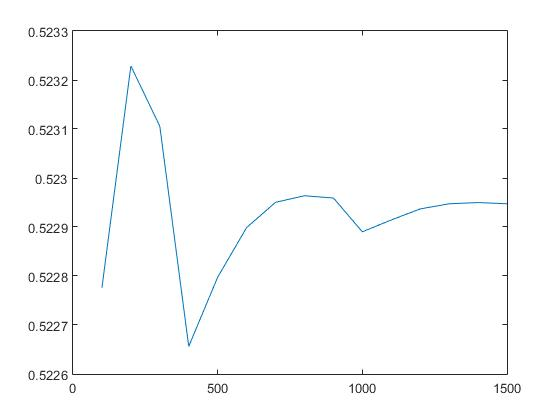
\includegraphics[scale=0.7]{smallPlot.jpg}
	\caption{European vanilla call option value estimates against $I$ with increments of 100}
\end{figure}

Since the value obtained at $I = 100$ is already quite close to the true value, it may be difficult to observe the convergence in the diagram of $I$ going from $100$ to $1500$ with increments of $100$ (figure 1). Hence, we plotted the diagram of $I$ going from $100$ to $1500$ with increments of $20$ in order to investigate further.

\begin{figure}[htbp!]
	\centering
	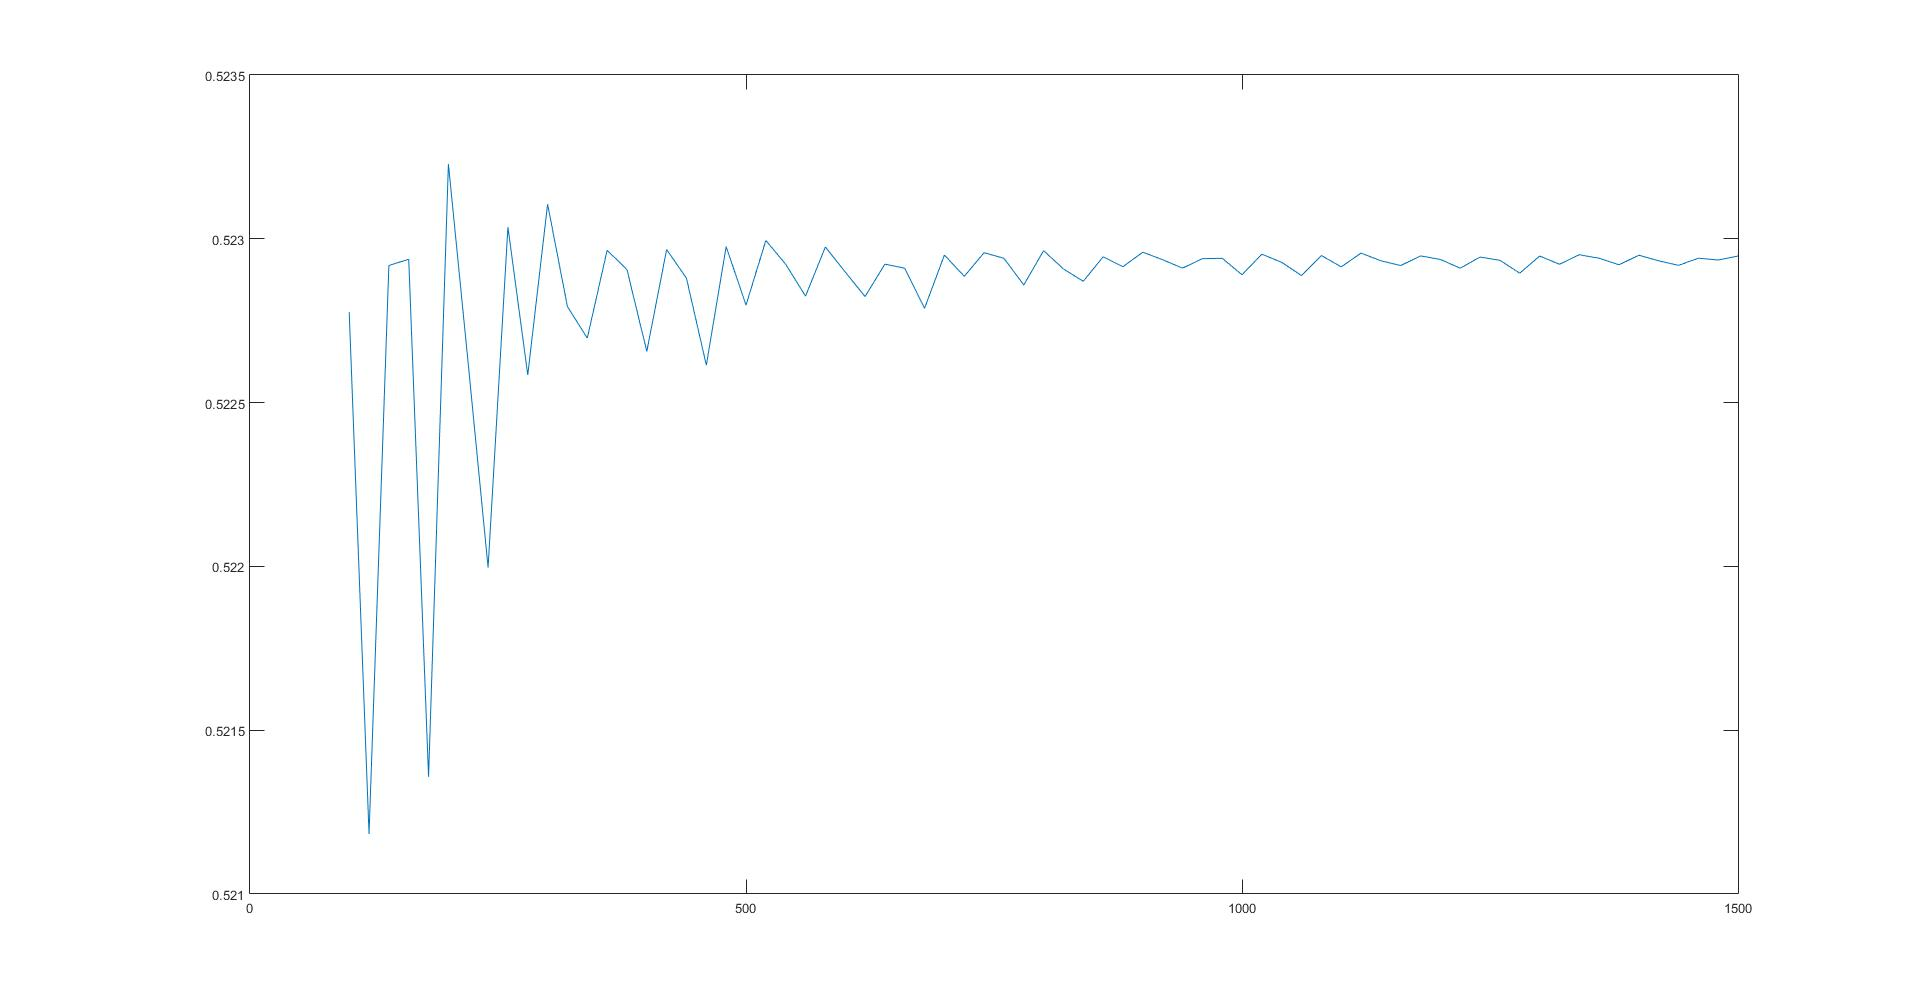
\includegraphics[scale=0.2]{largePlot.jpg}
	\caption{European vanilla call option value estimates against $I$ with increments of 20}
\end{figure}

From figure 2, it is obvious that the option value converges to the true value at around $\$0.52294$ as the fluctations become smaller and smaller as $I$ increases.

\subsection{American vanilla call option using PSOR}

For the American vanilla call option with same parameters as the above European vanilla call, we can use the projected SOR algorithm for the calculation of $U_{n}$ from $V_{n+1}$ with parameters $\epsilon = 1.0 * 10^{-6}, \omega = 1.3$.

\begin{center}
	\begin{tabular}{| c | c | c |}
		\hline $I$ & $N$ & Option price\\
		[0.5ex]
		\hline 100 & 1500 & 0.582849189993941 \\
		\hline 200 & 1500 & 0.583505358758593 \\
		\hline 300 & 1500 & 0.583457275858546 \\
		\hline 400 & 1500 & 0.582944640173874 \\
		\hline 500 & 1500 & 0.583166191075223 \\
		\hline 600 & 1500 & 0.583290840686203 \\
		\hline 700 & 1500 & 0.583345916640081 \\
		\hline 800 & 1500 & 0.583358092446549 \\
		\hline 900 & 1500 & 0.583351410333823 \\
		\hline 1000 & 1500 &0.583260621906101 \\
		\hline 1100 & 1500 &0.583286109957217 \\
		\hline 1200 & 1500 &0.583301049237271 \\
		\hline 1300 & 1500 &0.583302179614822 \\
		\hline 1400 & 1500 &0.583294042928569 \\
		\hline 1500 & 1500 &0.583280020736888 \\
		\hline
	\end{tabular}
\end{center}

We have plotted the values estimated with $I$ going from $100$ to $1500$ with increments of $100$ in figure 3.

\begin{figure}[htbp!]
	\centering
	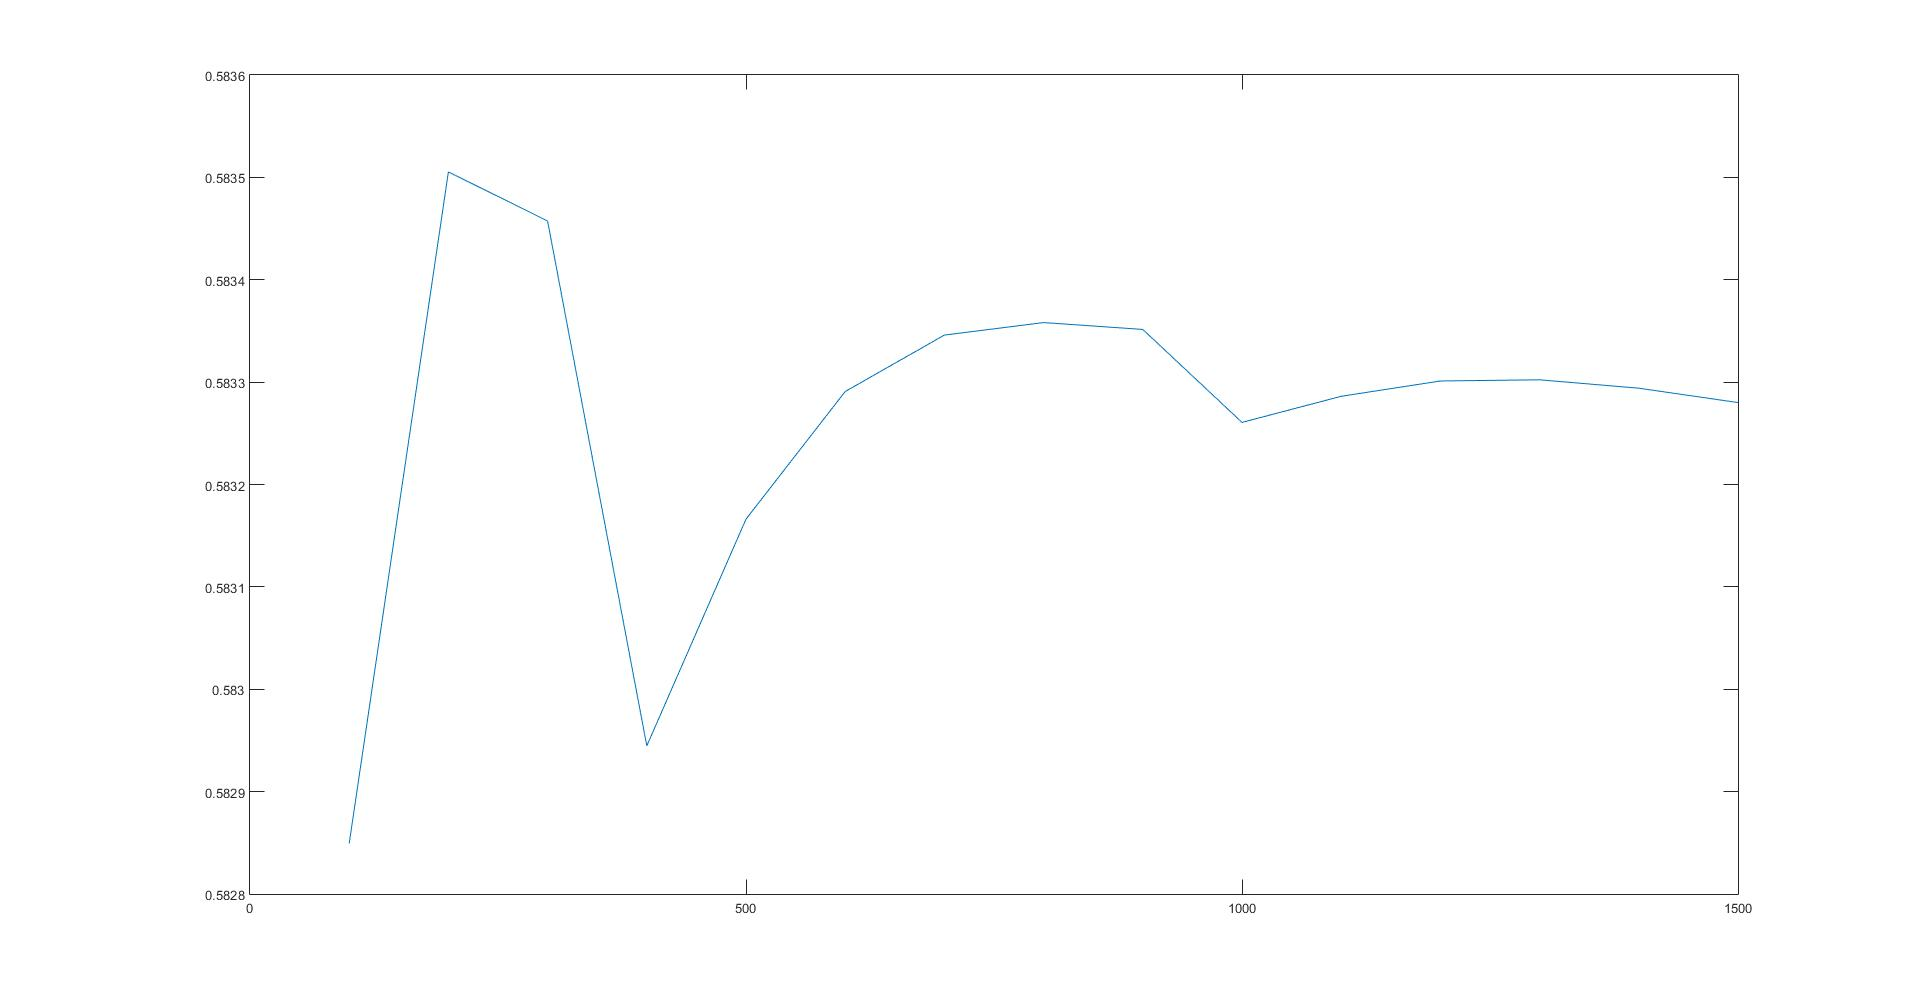
\includegraphics[scale=0.2]{smallPlot2.jpg}
	\caption{American vanilla call option value estimates against $I$ with increments of 100}
\end{figure}

Similar to the previous section, we plotted another diagram of $I$ going from $100$ to $1500$ with increments of $25$ in order to investigate further as figure 4.

\begin{figure}[htbp!]
	\centering
	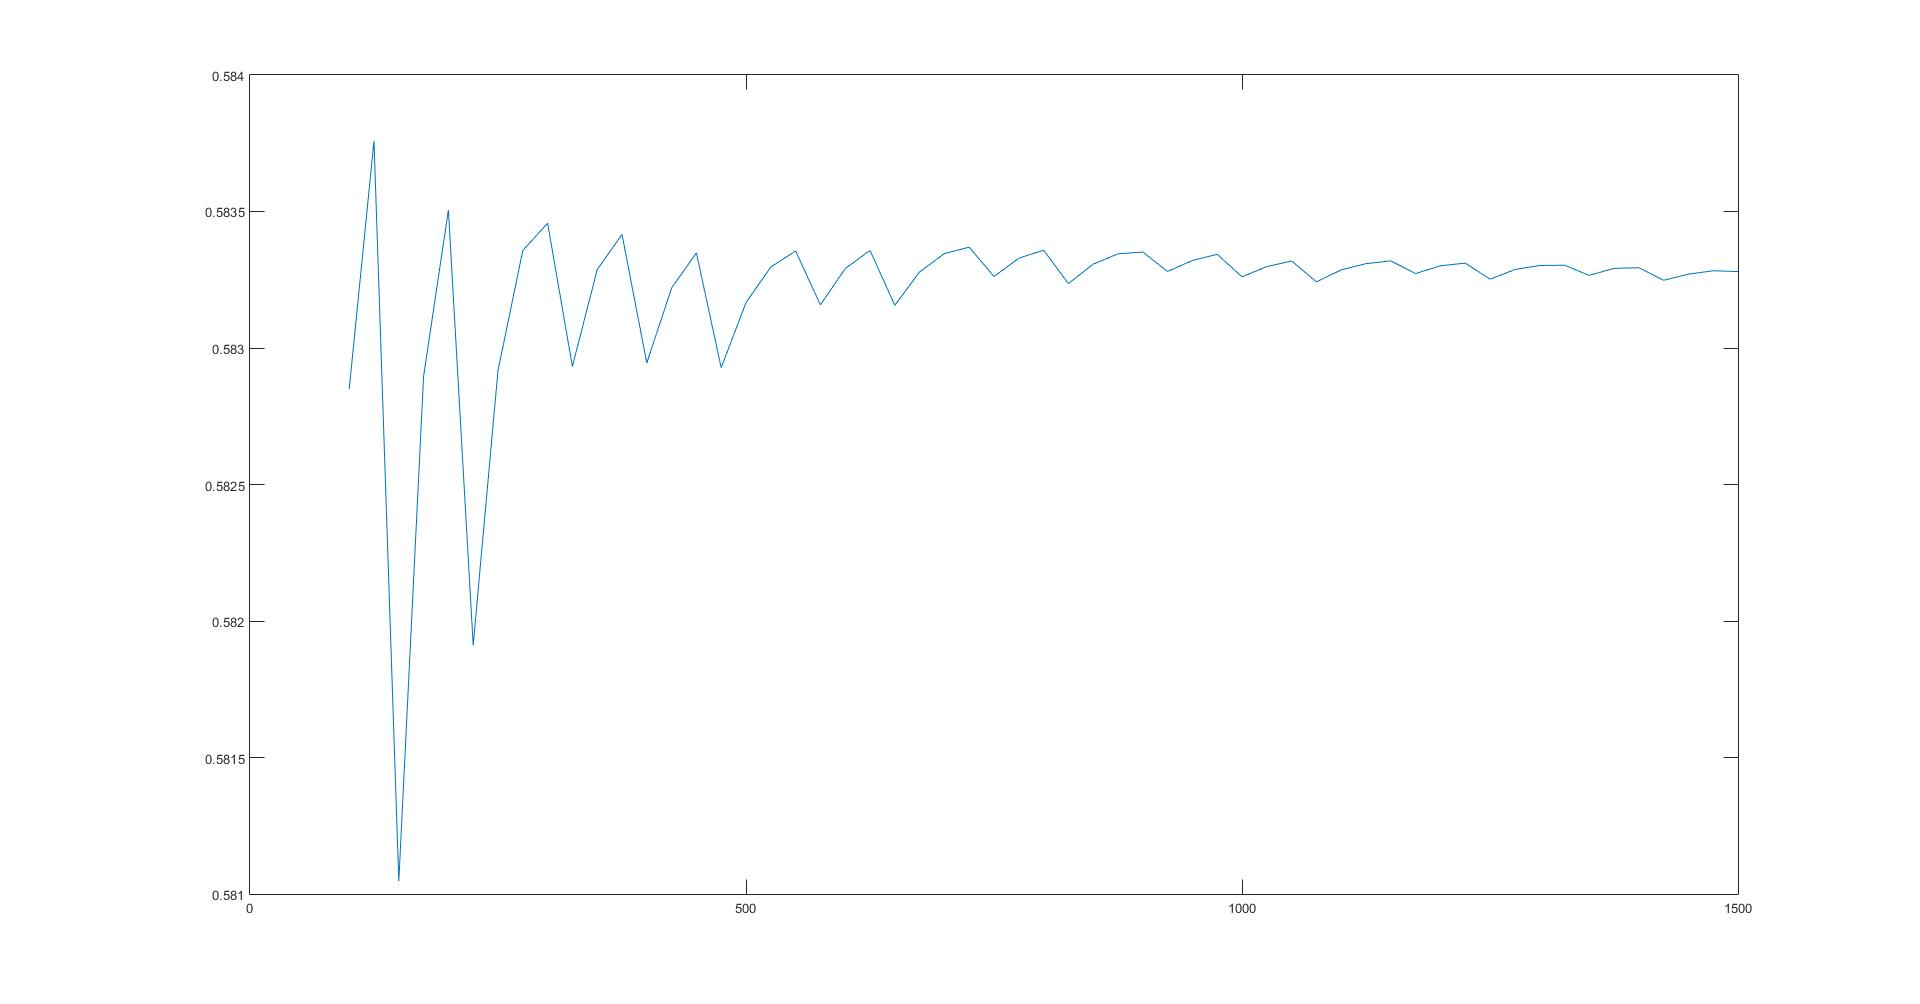
\includegraphics[scale=0.2]{largePlot2.jpg}
	\caption{American vanilla call option value estimates against $I$ with increments of 25}
\end{figure}

From figure 4, it is obvious that the option value converges to the true value at around $\$0.5834$ as the fluctations become smaller and smaller as $I$ increases.

\section{Valuation of digital call option}

\subsection{Pricing Algorithm of digital call option}

First, we implemented the function \texttt{BS\_DigitalCall(S0, X, r, q,  T, sigma)} for pricing the digital call option given:

\begin{algorithm}[H]
\setstretch{1.5}
	\KwData{$S_0$, $X$, $r$, $q$, $T$, $\sigma$}
	\KwResult{$c_{\text{DC}}$, Option Premium}
	$x = \dfrac{\log \left(\frac{S_0}{X}\right) + (r - q - \frac{\sigma^2}{2})T}{\sigma \sqrt{T}}$\;
	$c_{\text{DC}} = e^{-rT} N(x)$\;
\end{algorithm}

\subsection{Implementation of Monte Carlo Simulation without control variate}

Next up, we implemented the Monte Carlo simulation algorithm for estimating the 3-asset digital call option price, given the correlation matrix $C$ and the number of samples generated $N$, as well as the other parameters, $S_0$, $X$, $r$, $q$, $T$, same as those used in pricing of Digital Call option.

\begin{algorithm}[H]
\setstretch{1.5}
	\KwData{$S_0$, $X$, $r$, $q$, $T$, $\sigma$, $C$, $N$}
	\KwResult{$\texttt{MC\_noCV}$, Option Premium}
	\textit{First use the in-built function \emph{\texttt{randn}} in MATLAB to initiate a $3 \times N$ matrix \emph{$\mathbf{R}$.}} \\
	\textit{Each column of the matrix corresponds to the values of $x$ for the 3 assets in the portfolio.} \\
	$\mathbf{R} = \texttt{randn(3, N)}$\;
	\textit{Use Cholesky factorization to obtain a triangular matrix from the correlation matrix $C$} \\
	\textit{The in-build function \emph{\texttt{chol}} in MATLAB will lead to an upper triangular matrix.} \\
	$\mathbf{L} = \texttt{chol}(\mathbf{C})$ \;
	$\mathbf{E} =\mathbf{R}^T \mathbf{L} $ \;
	
	\textit{Construct the row matrix $\mathbf{p}$ for expected price.} \\
	\For {$j = 1,2,3$}{
		$\pmb{\mu}_j = r - \mathbf{q}_{j} - \frac{\pmb{\sigma}_{j}^2}{2}$ \;
		$\mathbf{p}_{j} = S_0 e^{\pmb{\mu}_jT}$ \;
	}
	\textit{Replicate the row matrices $\pmb{\sigma}$ and $\mathbf{p}$ into $N \times 3$ matrices $\mathbf{S}$ and $\mathbf{P}$} \\
	$\mathbf{S} = \texttt{repmat}(\pmb{\sigma}, N, 1)$ \;
	$\mathbf{P} = \texttt{repmat}(\mathbf{p}, N, 1)$ \;
	
	\textit{Thence, obtain the simulated terminal prices for the three assets, in an $N \times 3$ matrix $\mathbf{S}_T$.} \\
	\For {$i = 1 \dots N$}{
		\For {$j = 1,2,3$}{
			$w_{i,j} = \mathbf{S}_{i,j} \times \mathbf{E}_{i,j}$ \;
			$(\mathbf{S}_T)_{i,j} = \mathbf{p}_{i,j} \times\exp(w_{i,j}\sqrt{T})$
		}
	}
	
	\textit{Filter into a column matrix \emph{\texttt{max\_prices}} with only the maximum terminal prices in each sample.} \\
	$\texttt{max\_prices} = \texttt{max}(\mathbf{S}_T, \texttt{[]}, \texttt{2})$\;
	\textit{Filter out those in \emph{\texttt{max\_prices}} that are no more than strike $X$ into a column matrix \emph{\texttt{option\_values}}} \\
	$\texttt{option\_values} = (\texttt{max\_prices} > X)$ \;
	\textit{Finally, obtain the option value by discounting the average of the filtered terminal prices.} \\
	$\texttt{MC\_noCV} = \texttt{mean}(\texttt{option\_values}) \times e^{-rT}$ \;
	
\end{algorithm}

\subsection{Results from different number of price-path bundles and Comment}

Using the set of parameters, we obtain the following results in one of runs:

\begin{center}
	\begin{tabular}{| c | c | c | c |}
		\hline $X$ & $N$ & Option price estimate & Standard errors\\
		[0.5ex]
		\hline 8.5 & 30 & 0.86687 & 0.042158\\
		\hline 8.5 & 1000 & 0.87561 & 0.0095148\\
		\hline 8.5 & 10000 & 0.87745 & 0.0028249\\
		\hline 8.5 & 100000 & 0.87833 & 0.00081011\\
		\hline
		\hline 9.5 & 30 & 0.7149 & 0.089602\\
		\hline 9.5 & 1000 & 0.71379 & 0.014814\\
		\hline 9.5 & 10000 & 0.71402 & 0.0033345\\
		\hline 9.5 & 100000 & 0.71369 & 0.0013023\\
		\hline
		\hline 10.5 & 30 & 0.51049 & 0.088169\\
		\hline 10.5 & 1000 & 0.50082 & 0.013599\\
		\hline 10.5 & 10000 & 0.50434 & 0.0038309\\
		\hline 10.5 & 100000 & 0.50371 & 0.0013951\\
		\hline
	\end{tabular}
\end{center}

From the option price estimate for different strike prices, we do not observe an explicit overall increasing or decreasing trend. However, as $N$ gets larger, the change in estimated option price compared to the previous value of $N$ gets to decrease. 

This trend is more evidenced in the value of standard errors, which effectively decreased from smaller values of $N$ to larger values. Each time when $N$ increased by $10$ times, the value of standard errors is lowered to approximately between $\dfrac{1}{4}$ to $\dfrac{1}{3}$ of the previous value, which is similar to the value of $\dfrac{1}{\sqrt{10}}$.


\subsection{Variance Control and Effectiveness}


\end{document}